\section{Ein würdiger Abschluss und ein Blick nach vorn}


Liebe Leserin, lieber Leser,

herzlichen Glückwunsch! Du hast dich durch eine beachtliche Menge an mathematischen Konzepten gearbeitet, von den alltäglichen Grundlagen des Dreisatzes bis zu den anspruchsvollen Gipfeln der Differential- und Integralrechnung, und dabei auch die faszinierenden Welten der Exponential- und Logarithmusfunktionen erkundet. Das ist eine beeindruckende Leistung, die Ausdauer, Neugier und eine gehörige Portion Gehirnschmalz erfordert hat!

\begin{center}
    \Large\bfseries Hut ab vor deinem Durchhaltevermögen!
\end{center}
\vspace{1em}

Du hast nicht nur Formeln und Rechenwege kennengelernt, sondern hoffentlich auch ein tieferes Verständnis für die Struktur und die innere Logik der Mathematik entwickelt. Du hast gesehen, wie verschiedene Ideen miteinander verwoben sind:
\begin{itemize}
    \item Wie der einfache Dreisatz die Grundlage für das Verständnis linearer Zusammenhänge legt.
    \item Wie lineare Funktionen uns zu den eleganteren Kurven der quadratischen Funktionen führen.
    \item Wie die Differentialrechnung uns erlaubt, Veränderungen präzise zu beschreiben – von der momentanen Geschwindigkeit bis zur optimalen Form eines Kaffeefilters.
    \item Wie die Integralrechnung uns die Macht gibt, aus Änderungsraten Gesamtgrößen zu rekonstruieren und Flächen unter Kurven zu bestimmen, die vorher unerreichbar schienen.
    \item Und wie Exponential- und Logarithmusfunktionen uns helfen, die dynamischen Prozesse des Wachstums und Zerfalls in der Welt um uns herum zu modellieren.
\end{itemize}

\begin{infoboxumgebung}{Mehr als nur Zahlen und Formeln}
Mathematik ist, wie du vielleicht gemerkt hast, viel mehr als nur das Rechnen mit Zahlen. Sie ist eine Sprache, die uns hilft, die Welt präzise zu beschreiben, Muster zu erkennen, Probleme zu lösen und logische Schlüsse zu ziehen. Die Werkzeuge, die du in diesem Skript kennengelernt hast, sind fundamental – nicht nur für weitere mathematische Studien, sondern auch für unzählige Anwendungen in den Naturwissenschaften, der Technik, der Wirtschaft, der Informatik und vielen anderen Bereichen.

Denke an die Eleganz der Eulerschen Zahl $e$, die wie von Zauberhand in Wachstumsprozessen und bei kontinuierlicher Verzinsung auftaucht, oder an die Art und Weise, wie Sinus und Kosinus die periodischen Rhythmen der Natur einfangen. Die Fähigkeit, solche Zusammenhänge zu verstehen und mathematisch zu modellieren, ist eine wertvolle Kompetenz.
\end{infoboxumgebung}

\begin{warumwichtigumgebung}{Dein mathematischer Werkzeugkasten ist jetzt gut gefüllt!}
Mit dem Wissen aus diesem Skript bist du nun in der Lage:
\begin{itemize}
    \item Lineare und quadratische Gleichungen und Funktionen sicher zu handhaben.
    \item Die Grundkonzepte der Differentialrechnung (Ableitung, Ableitungsregeln) zu verstehen und anzuwenden.
    \item Vollständige Kurvendiskussionen für Polynomfunktionen sowie für grundlegende Exponential- und Logarithmusfunktionen durchzuführen.
    \item Die Grundlagen der Integralrechnung (Stammfunktion, bestimmtes Integral, Hauptsatz) zu verstehen und für Flächenberechnungen und einfache Anwendungen zu nutzen.
    \item Die besonderen Eigenschaften und Anwendungsfelder von Exponential- und Logarithmusfunktionen zu erkennen.
\end{itemize}
Das ist ein solides Fundament, auf dem du aufbauen kannst, sei es im weiteren Schulverlauf, im Studium oder einfach aus persönlichem Interesse.
\end{warumwichtigumgebung}

\textbf{Wie geht es weiter?}

Die Reise durch die Mathematik ist nie wirklich zu Ende. Es gibt immer neue, spannende Gebiete zu entdecken. Basierend auf dem, was wir hier behandelt haben, könnten nächste Schritte sein:
\begin{itemize}
    \item \textbf{Vertiefung der Integrationstechniken:} Neben der partiellen Integration und Substitution gibt es weitere Methoden, um komplexere Integrale zu lösen.
    \item \textbf{Vektorrechnung und Analytische Geometrie:} Die Beschreibung von Punkten, Geraden und Ebenen im Raum.
    \item \textbf{Stochastik (Wahrscheinlichkeitsrechnung und Statistik):} Die Mathematik des Zufalls und der Datenanalyse.
    \item \textbf{Komplexe Zahlen:} Eine Erweiterung des Zahlenbereichs, die in vielen Bereichen der Physik und Technik unerlässlich ist.
    \item \textbf{Differentialgleichungen:} Gleichungen, die Funktionen und ihre Ableitungen beinhalten und zur Modellierung dynamischer Systeme dienen.
\end{itemize}
Lass deine Neugier dein Kompass sein!

\begin{tippumgebung}{Bleib am Ball!}
Der Schlüssel zum Erfolg in der Mathematik ist kontinuierliche Übung und die Bereitschaft, sich auch mit herausfordernden Problemen auseinanderzusetzen. Nutze die Aufgaben in diesem Skript, suche dir weitere Übungen, arbeite mit Mitschülern zusammen und scheue dich nicht, Fragen zu stellen.

Denke daran: Jeder Fehler ist eine Chance zu lernen. Die Aha-Momente, wenn ein komplexer Zusammenhang plötzlich klar wird, sind die schönste Belohnung. \smiley{}
\end{tippumgebung}

\begin{funfactbox}{Der Zick-Zack-Tanz der Moleküle: Wenn $(\Delta \text{Weg})^2$ plötzlich zählt!}
Du kennst die Brownsche Bewegung vielleicht aus dem Physik- oder Chemieunterricht: die unaufhörliche, zufällige Zitterbewegung winziger Teilchen (z.B. Pollen auf einer Wasseroberfläche), die durch die Stöße der umgebenden Moleküle verursacht wird. Albert Einstein lieferte 1905 eine bahnbrechende theoretische Erklärung für dieses Phänomen, die half, die Existenz von Atomen und Molekülen endgültig zu beweisen!

Der Pfad eines solchen Teilchens, $W_t$ zur Zeit $t$, ist extrem unregelmäßig und zackig – so sehr, dass er mathematisch gesehen an keinem einzigen Punkt differenzierbar (also 'glatt') ist! Diese extreme 'Rauheit' führt zu erstaunlichen Eigenschaften.

Stell dir vor, du betrachtest eine 'normale', glatte Funktion $f(t)$, z.B. den Weg eines gleichmäßig beschleunigten Objekts. Wenn du die Änderungen $\Delta f = f(t_{i+1}) - f(t_i)$ über viele kleine Zeitintervalle $\Delta t = t_{i+1} - t_i$ betrachtest, dann gilt $\Delta f \approx f'(t_i) \Delta t$. Wenn du nun die Quadrate dieser Änderungen aufsummierst, $\sum (\Delta f)^2 \approx \sum (f'(t_i))^2 (\Delta t)^2$, und die Zeitschritte $\Delta t$ immer kleiner machst, geht diese Summe sehr schnell gegen Null (wegen des $(\Delta t)^2$).

\textbf{Die Überraschung bei der Brownschen Bewegung:}
Bei der Brownschen Bewegung $W_t$ ist das anders! Wenn man die Quadrate der Wegänderungen $\Delta W_i = W_{t_{i+1}} - W_{t_i}$ über kleine Zeitintervalle $\Delta t$ aufsummiert, passiert etwas Unerwartetes:
\[ \sum_{i=0}^{N-1} (W_{t_{i+1}} - W_{t_i})^2 \quad \text{für } t_0=0, t_N=T \text{ und } \Delta t = T/N \]
Wenn man die Zeitintervalle $\Delta t$ immer kleiner macht ($N \to \infty$), geht diese Summe nicht etwa gegen Null, sondern sie nähert sich dem Gesamtwert der verstrichenen Zeit $T$ an!
\[ \lim_{\Delta t \to 0} \sum (W_{t_{i+1}} - W_{t_i})^2 = T \]
Dieses Ergebnis nennt man die \textbf{quadratische Variation} der Brownschen Bewegung. Es bedeutet heuristisch, dass $(dW_t)^2$ sich wie $dt$ verhält – das Quadrat einer winzigen Änderung des Weges ist so groß wie die winzige Änderung der Zeit! Das ist völlig anders als bei glatten Funktionen, wo $(df)^2 \approx (f'(t)dt)^2$ ein Term 'höherer Ordnung' ist, der viel schneller verschwindet.

Diese besondere Eigenschaft $E[(dW_t)^2] \approx dt$ (wobei $E[\dots]$ für den Erwartungswert steht, eine Art Mittelwert über viele mögliche Pfade) ist einer der Gründe, warum für die Beschreibung von Zufallsprozessen eine eigene, spezielle Form der Analysis entwickelt wurde, die sogenannte \textbf{stochastische Analysis} (oder Itô-Kalkül). Sie spielt heute eine riesige Rolle, z.B. in der Finanzmathematik bei der Modellierung von Aktienkursen. Was als Beobachtung von zitternden Pollen begann, hat also zu ganz neuen mathematischen Welten geführt!

\begin{center}
    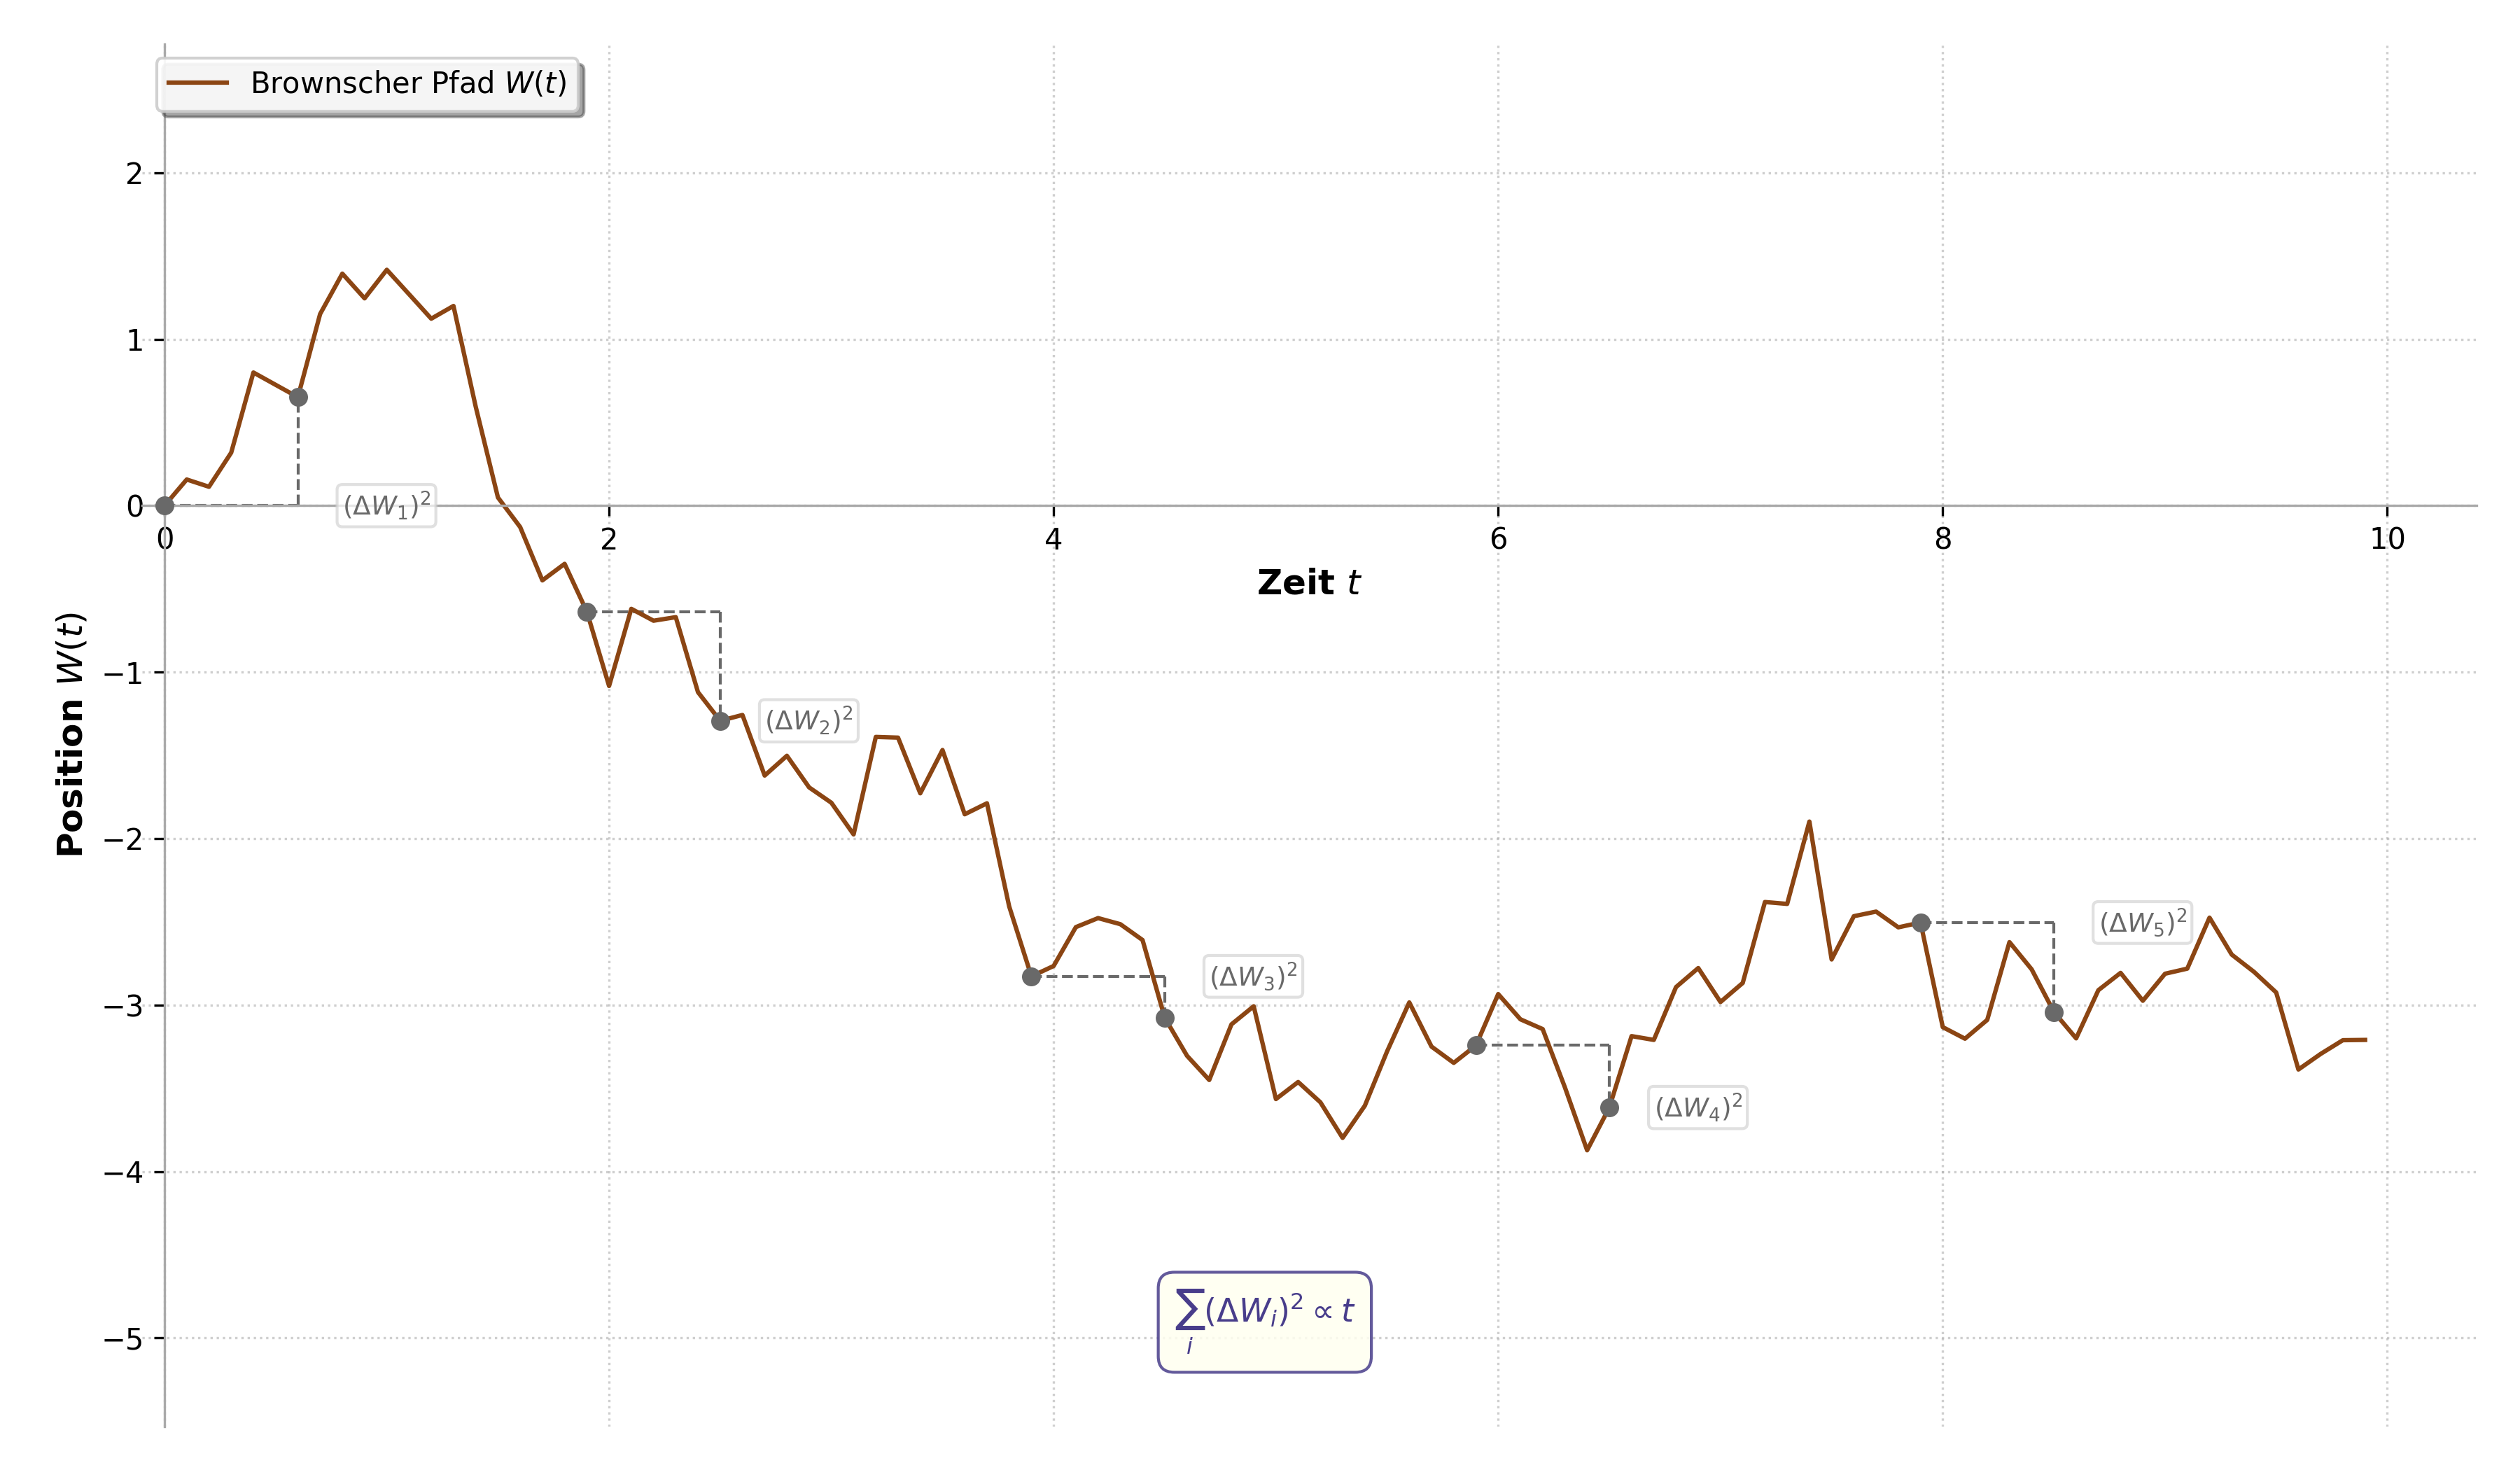
\includegraphics[width=0.7\textwidth]{grafiken/Brownsche_Bewegung_QV.png}
    % Beschreibung für die Grafik 'Brownsche_Bewegung_QV.png':
    % Die Grafik könnte schematisch einen stark zackigen Pfad einer Brownschen Bewegung zeigen.
    % Entlang des Pfades könnten kleine Segmente markiert sein, deren Längenquadrate 
    % (Delta W_i)^2 symbolisch dargestellt werden.
    % Eine Achse könnte die Zeit 't' darstellen.
    % Vielleicht eine kleine Sprechblase: 'Summe der (Delta Weg)^2 ist proportional zur Zeit!'
    \captionof{figure}{Konzept der quadratischen Variation bei der Brownschen Bewegung}
    \label{fig:brownsche_bewegung_qv_funfact}
\end{center}
\end{funfactbox}

Wir hoffen, dieses Lernmaterial hat dir nicht nur Wissen vermittelt, sondern auch ein wenig von der Faszination und der Schönheit der Mathematik gezeigt. Die Fähigkeit, logisch zu denken, Probleme strukturiert anzugehen und komplexe Zusammenhänge zu durchdringen, wird dir in vielen Lebensbereichen von Nutzen sein.

\vspace{1em}
\begin{center}
    \Large\itshape Alles Gute auf deinem weiteren Weg!
\end{center}
\vspace{2em}

% Ende des Anhangs-Kapitels
